\bgroup{}

\chapter{Implementation}\label{cha:implementation}
In order to present audio tagging with subjective labels in practice, the author of this thesis has built an application that strives to minimize the manual tagging effort needed by a user. Although simplistic, the application is a functional demonstration of how these problems could be solved using existing technologies, combining them into a solution. This chapter explains the design of the program, presents an overview of how the logic works, and examines implementation-specific problems.

\section{System architecture}
All of the codebase for the application uses \emph{Python}~\cite{python}, mostly due to it being a widely-used programming language for scientific purposes~\cite{python:survey}, along with having an extensive number of \gls{ml} and \gls{ai} packages accessible for use~\cite{python:about}. At the time of writing, version 3.8.1 is the latest stable release, which is also the version used throughout the codebase.

Some additional packages assist with certain functionalities:
\begin{itemize}
    \item \emph{AudioCommons Timbral Models}~\cite{timbral_models} analyzes sound input, calculates timbral attributes, and outputs the result to a usable data format.
    \item \emph{scikit-learn}~\cite{scikit-learn}, along with \emph{NumPy}~\cite{numpy}, is used for the sound similarity estimation part of the application.
    \item \emph{TinyDB}~\cite{tinydb} handles elements related to databases.
    \item \emph{pipenv}~\cite{pipenv} installs and manages packages used in the project in a virtual environment.
    \item \emph{autopep8}~\cite{autopep8}, \emph{pylint}~\cite{pylint}, and \emph{rope}~\cite{rope} deal with formatting, linting, and refactoring, respectively.
\end{itemize}
The straightforward, yet representative, \gls{ui} utilizes the \emph{tkinter}~\cite{tkinter} package as its infrastructure. This package is included in most \emph{Python} distributions by default and offers a decent toolkit to make \glspl{gui}.
\begin{figure}[ht]
    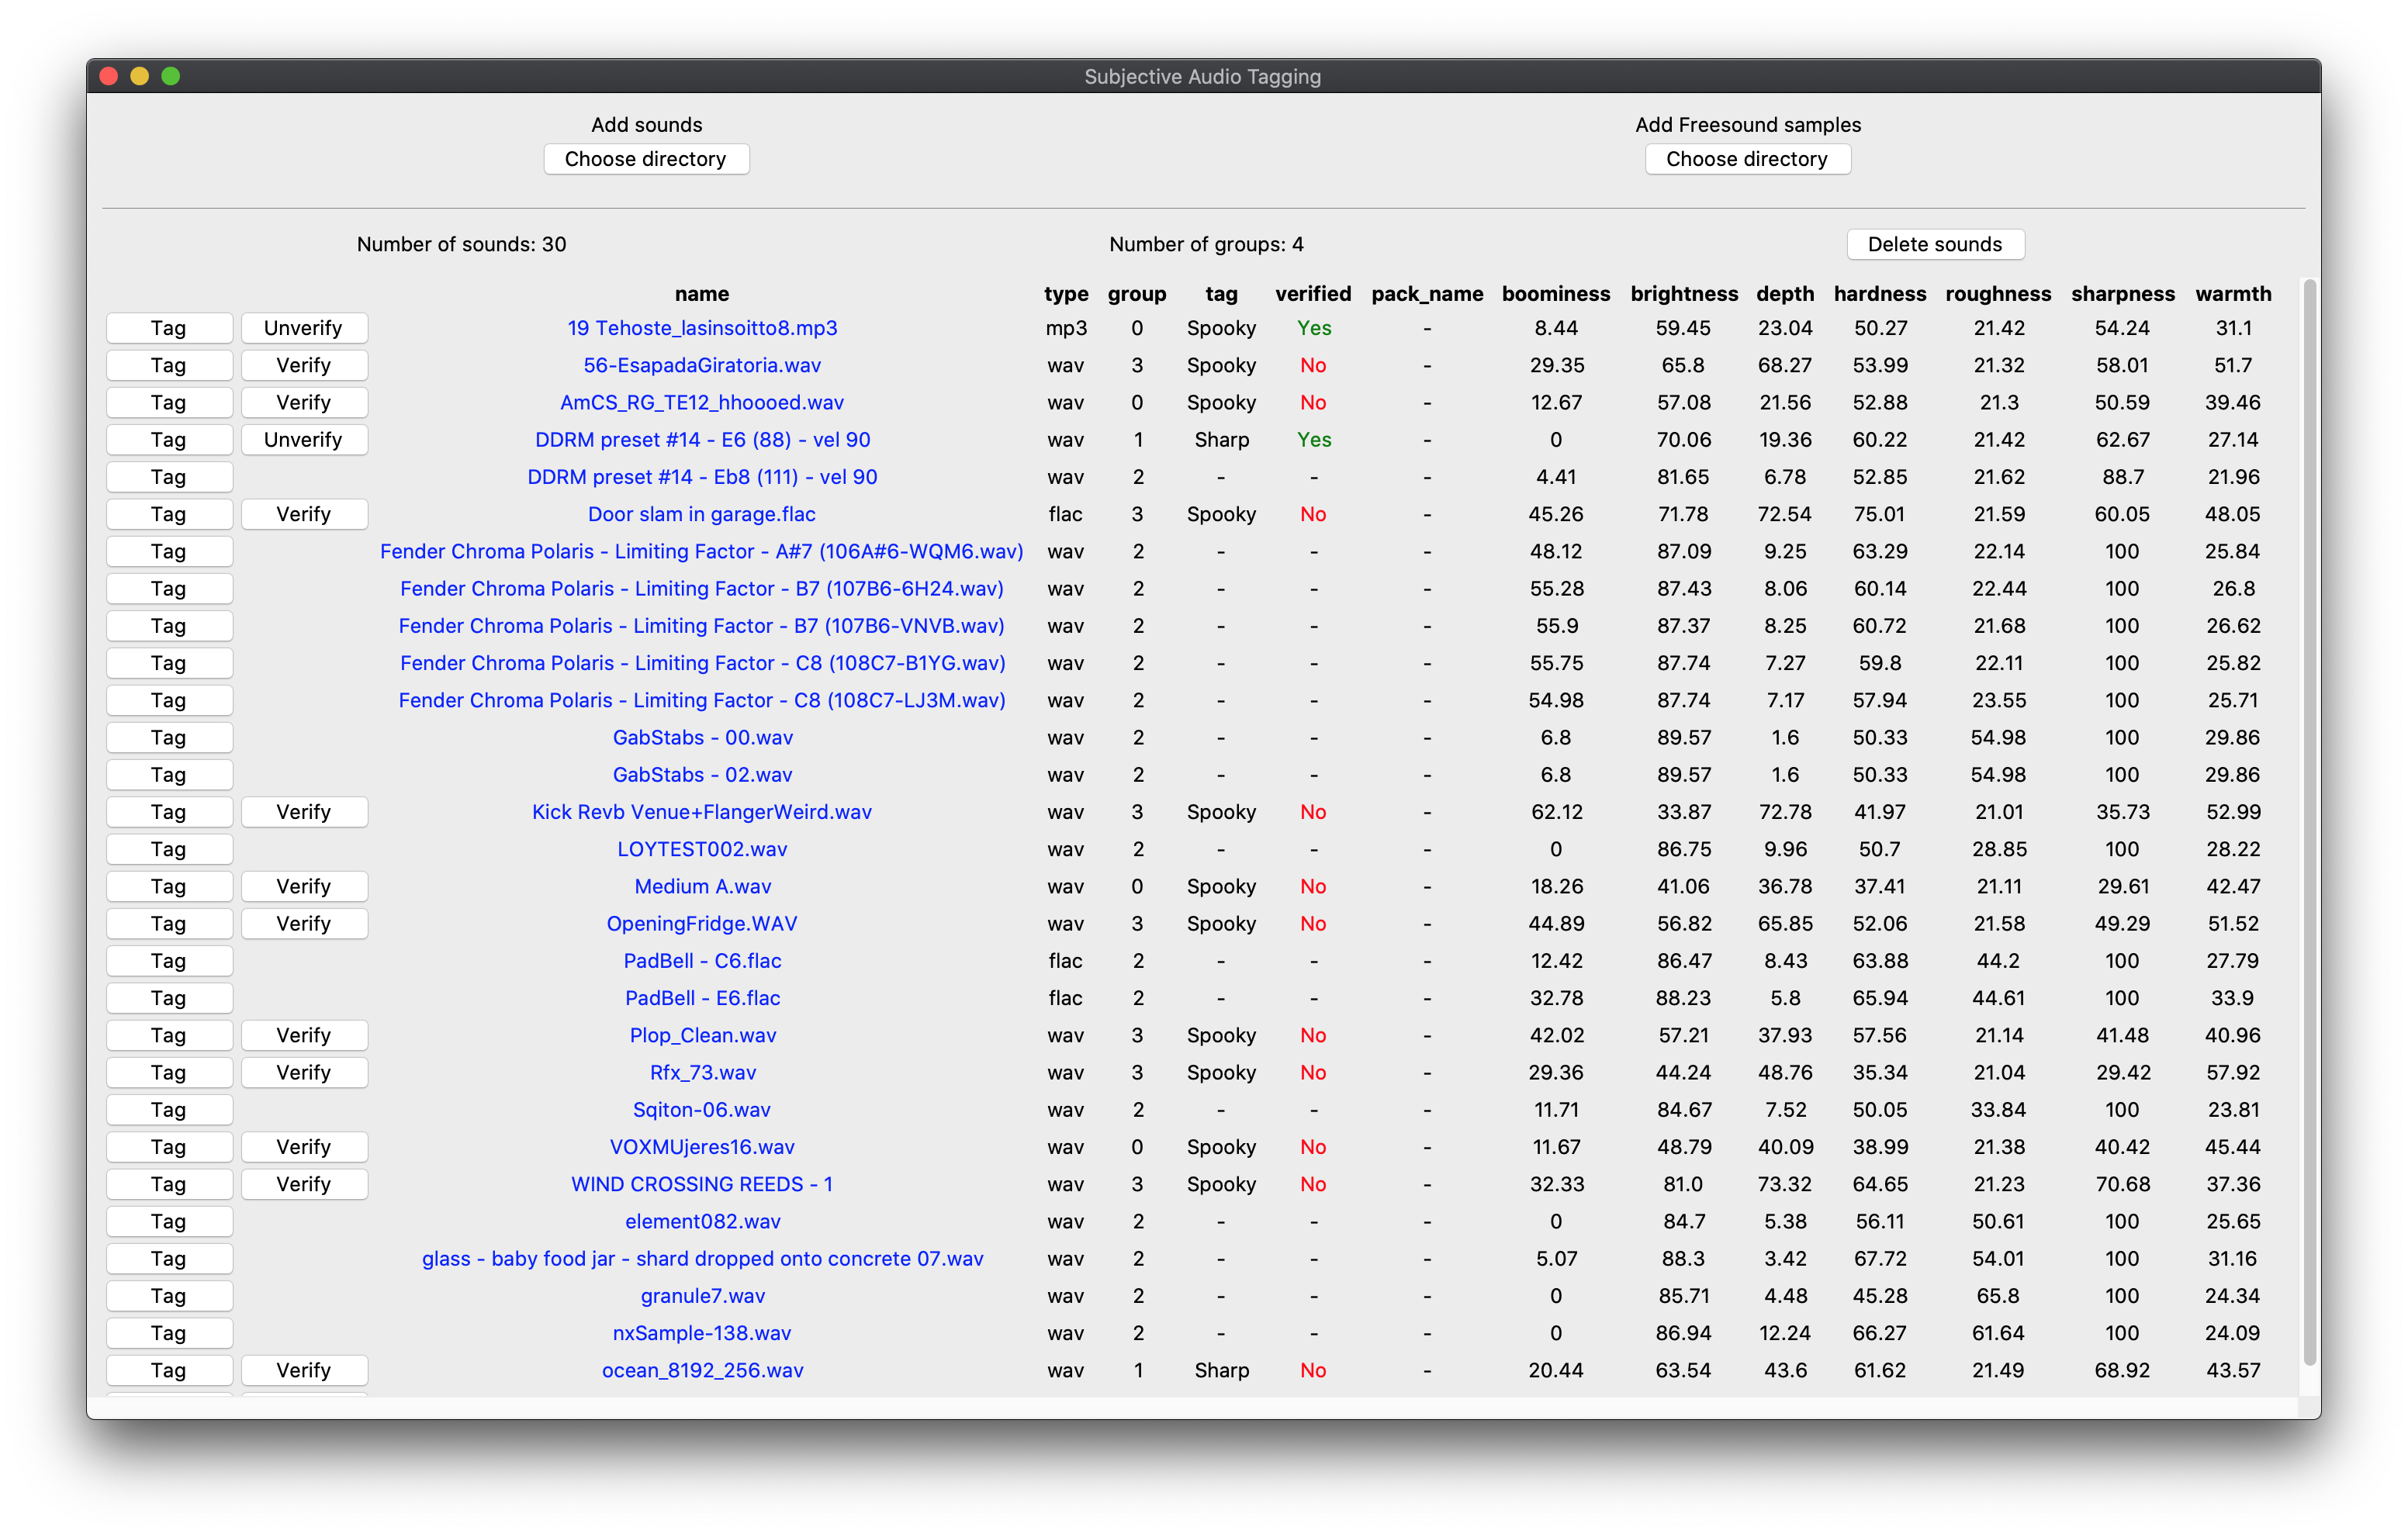
\includegraphics[width=\textwidth]{figures/app/ui}
    \caption{\glsentrytext{ui} of the application.}\label{fig:app/ui}
\end{figure}
\begin{mdframed}[style=info]
    \textbf{NB} Although the \gls{ui} is an essential and necessary part of an application, the priority of it has been lowered in this project to allow more time spent on calculation-heavy parts of the program.
\end{mdframed}

\section{Overview}
By looking at \cref{fig:app/ui}, one can see that the application consists of an upper and a lower section. Clicking the buttons in the upper section adds sounds to the application in one of two different ways, processing them accordingly (described in \cref{sec:adding_sounds} and \cref{sec:sound_similarity}). In the lower section, an info-panel displays statistics about all sounds added, plus a delete-all button, and a table underneath shows metadata for the sounds. Alongside the attributes shown, each row also lists buttons used for updating a particular sound. In conjunction with the possibility of listening to a sound by clicking its highlighted name, these buttons allow for tagging and verifying of sounds (\cref{sec:tagging}). The user can also choose to rename a tag or, after the program has assigned its tags, discard a tag, and relabel a sound entirely (\cref{sec:automatic_tagging}). Finally, some additional logic is required when adding more sounds to the application, but once done, the user can repeat all of the previously mentioned steps (\cref{sec:additional_sounds}).

\section{Adding sounds}\label{sec:adding_sounds}
The process of adding sounds to the application starts when the user clicks the upper leftmost button in \cref{fig:app/ui} and chooses a directory that contains audio files; the implementation supports many of the most commonly used audio formats. However, before the sounds appear in the \gls{ui} where they can be tagged, they first have to be analyzed and converted to a usable format.

\emph{AudioCommons Timbral Models} is a package that processes sounds and predicts eight timbral characteristics, which in turn helps managing sounds and enables measuring and comparison between them. The `semantic annotation of non-musical sound properties' work package deliverables explain how these characteristics were developed and describe the implementation of the models, plus usage of the package in detail~\cite{rep:d5.1, rep:d5.2, rep:d5.3, rep:d5.6, rep:d5.7, rep:d5.8}. Although developed to aid with automatic tagging of sounds~\cite[4]{rep:d5.8}, in this project, the calculated attributes distinguish one sound from another regarding similarity.

The eight timbral characteristics are:
\begin{enumerate}
    \item \emph{booming}
    \item \emph{brightness}
    \item \emph{depth}
    \item \emph{hardness}
    \item \emph{roughness}
    \item \emph{sharpness}
    \item \emph{warmth}
    \item \emph{reverberation}
\end{enumerate}
The seven first characteristics are all regression-based models. These models produce a numerical output ranging from 0 to 100; the \texttt{clip\_output} parameter seen in \cref{lst:process_sounds} restrains the upper value, as it may otherwise exceed the range. The last feature, \emph{reverberation}, is a classification model, producing a boolean value represented as 0 or 1.
Since the output values serve as a measurement for how similar sounds are – computed by \gls{ml} algorithms – each one of them is considered equally significant. However, as the \emph{reverberation} model produces a different ranging result, the prerequisite for a homologous environment rules it out. Therefore, the program omits the \emph{reverberation} value (shortened to \emph{reverb} in the function output) when processing added sounds.
\begin{mdframed}[style=code]
    \lstinputlisting[firstline={50},caption={Function for processing (nested) sounds in a directory.},label={lst:process_sounds}]{../app/logic/timbral_models.py}
\end{mdframed}

\subsection{Freesound samples}
As seen from \cref{fig:app/ui}, there are two buttons in the upper section for adding sounds to the application. The alternative rightmost button accepts predefined \emph{Freesound}~\cite{freesound} metadata files, i.e., \gls{json} files with the timbral characteristics included. Because \emph{Freesound} integrates with the \emph{Audio Commons Audio Extractor}~\cite{ac-audio-extractor} tool (which uses the same timbral prediction as \emph{AudioCommons Timbral Models}), almost all available sounds have an associated metadata file containing the calculated timbral attributes~\cite{freesound:integration}. To browse and download these files, one can use the \emph{Freesound API}~\cite{freesound:api} or the \emph{Audio Commons Extractor Web Demonstrator}~\cite{ac-audio-extractor:web_demonstrator}. This feature makes it possible to add sets of biased data, namely where the wanted result is defined; the tests in the evaluation chapter (\cref{cha:evaluation}) uses these constructed sets when measuring results. It also speeds up the process of experimenting with different sounds, as the analysis of sounds done by the \emph{AudioCommons Timbral Models} package can be slow at times, especially for larger audio files.
\begin{mdframed}[style=code]
    \lstinputlisting[firstline={18},lastline={48},caption={Function for processing Freesound samples.},label={lst:process_freesound_samples}]{../app/logic/timbral_models.py}
\end{mdframed}

\subsection{Deleting sounds}
A possibility to delete sounds is available in the application by clicking the pertinently named button displayed in \cref{fig:app/ui}. This interaction opens a prompt where the user confirms the choice to remove all sounds. If approved, all databases purge their content, and the program returns to its initial state.

\section{Sound similarity}\label{sec:sound_similarity}
The timbral characteristics described in \cref{sec:adding_sounds} estimates the similarity of sounds in this project. When comparing two sounds, the more closely resembling predicted timbral values there are between them, the more similar the sounds are. The \gls{ml} logic uses this estimation of closeness when finding groups of sound, or \emph{clusters}. All sounds in a cluster link to a single tag; multiple clusters can have the same tag.

\subsection{Mean shift}\label{sub:mean_shift}
Two different \gls{ml} algorithms operate together in the application to find and maintain groups of sound. Both of them come from the \emph{scikit-learn} package. The first algorithm searches for naturally occurring clusters in a set of data using the \emph{Mean shift}~\cite{mean_shift} procedure. It operates on the timbral coordinates for all sounds, \(X\), and produces an array of cluster centers, also called \emph{centroids}. Since the final sum of tags a user chooses to use throughout the application is unknown, \emph{Mean shift} works particularly well for creating a foundation of how many groups of sound could be satisfactory. It independently decides on the optimal number of centroids in a set of data, making it ideal for creating a starting point.
\begin{mdframed}[style=code]
    \lstinputlisting[firstline={37},lastline={44},caption={Function for finding initial clusters.},label={lst:init_groups}]{../app/logic/machine_learning.py}
\end{mdframed}

\subsection{K-means}\label{sub:k-means}
\emph{K-means}~\cite{k-means} is the second \gls{ml} algorithm used for calculating clusters among sounds. This algorithm is the method used to separate the sounds into different groups and marking them accordingly. It takes as input the current cluster center coordinates, which are either produced by the preparatory \emph{Mean shift} procedure or by a previous iteration of the \emph{K-means} clustering. These coordinates guide the algorithm when deriving renewed concluding centroids. It also needs a \(k\) value, which is the number of groups to split the data in, derived from the number of centroids. Lastly, the \texttt{n\_init} parameter tells the algorithm to perform a single iterator on each seed, so the new cluster center coordinates do not strive too far from the previously calculated ones. Like the \emph{Mean shift} algorithm, the \emph{K-means} procedure operates on \(X\), being coordinates for the timbral characteristics of all sounds. As the number of tags and groups grows with usage, this algorithm scales proportionately and, when executed, produces the correct updated number of centroids.
\begin{mdframed}[style=code]
    \lstinputlisting[firstline={22},lastline={35},caption={Function for finding groups of sound.},label={lst:find_groups}]{../app/logic/machine_learning.py}
\end{mdframed}

\subsection{Usage}
Each time the user adds a set of sounds to the application, both the \emph{Mean shift} and the \emph{K-means} algorithm invokes in sequence. This step makes sure that every sound added belongs to a group, and if applicable, tags additional sounds with the existing group's tag. Whenever there is a need for a new group (described in \cref{sub:modifying_groups}), the \emph{K-means} algorithm is triggered separately.

\section{Tagging}\label{sec:tagging}
\begin{figure}[ht]
    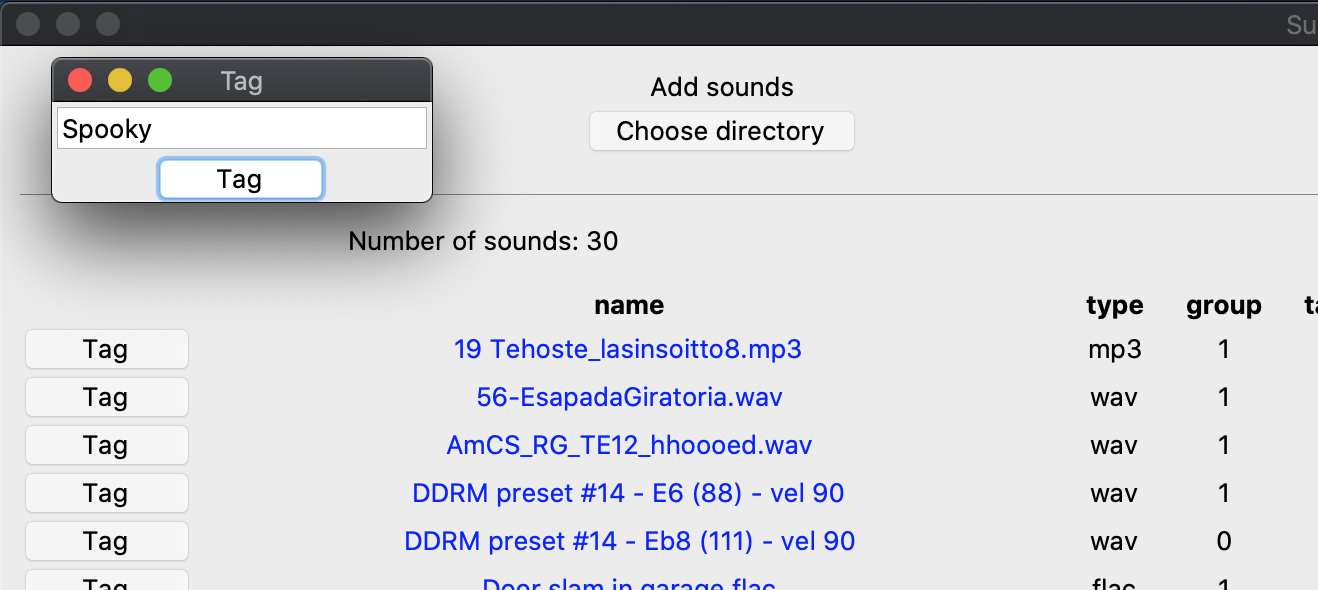
\includegraphics[width=\textwidth]{figures/app/tagging}
    \caption{Tagging a sound.}\label{fig:app/tagging}
\end{figure}
Once sounds have been processed, designated to a group, and added to the application, the user can start tagging them. To annotate a sound with a tag, the user clicks the corresponding button in the table and fills in the subsequent dialog, illustrated in \cref{fig:app/tagging}. The label the user chooses to enter in the dialog can be the same as an existing tag or a new one. The sound's \emph{tag} property – which is declared empty in both \cref{lst:process_sounds} and \cref{lst:process_freesound_samples} – stores this input value. To decide what tag goes along with a sound, the user probably wants to listen to the sound first. The sound names listed in the table shown in \cref{fig:app/ui} are links that trigger this action, opening the matching audio file in the system default application.
\begin{mdframed}[style=info]
    \textbf{NB} The implementation limits tagging to allow only a single label per sound; multiple groups can have the same tag. This restriction scales down the logic and code needed for the application, especially in the \gls{ml} parts.
\end{mdframed}

\subsection{Verification}
For the user to be able to keep track of which sounds they have tagged, each sound has a \emph{verified} property. This attribute is a boolean flag initially set to \texttt{False} for all sounds, established in \cref{lst:process_sounds} and \cref{lst:process_freesound_samples}. Whenever the user tags a sound, the \emph{verified} status remains or changes to \texttt{True} for that sound, as opposed to the automatic tagging process by the program, which will not affect the value of the property. When a sound has a tag – assigned either manually or automatically – the user can choose to toggle the \emph{verified} status by clicking the corresponding button in the table (see \cref{fig:app/ui}). The \emph{verified} property also determines how the automatic tagging behaves, judging the need to create new groups or carry on with the ones already defined.

\section{Automatic tagging}\label{sec:automatic_tagging}
One of the core functionalities in the application is the inclusion of an automatic tagging system. This procedure helps cut down the overall effort needed to label sounds and is flexible enough to cover most use cases adequately. For every sound manually tagged by the user, the program responds by automatically tagging similar sounds. The logic consists of two different operations, where the selection of the alternative to execute is dependent on the relevant sound's \emph{verified} property. One option directly changes a group's tag, or in other words, performs a tag renaming. The other is slightly more complex, creating one or more new groups and modifying existing tags and groups. Both alternatives save the modifications to the application databases and repaint the screen with the revised sounds once done.

\subsection{Tag renaming}
The first and more straightforward of the two automatic tagging scenarios is a renaming of a group's tag where all ongoing groupings are kept intact. This event triggers when a \emph{verified} sound is tagged, or when the user tags a sound belonging to a group where all sounds lack verification. The latter happens, for instance, when the user tags a sound for the first time since all sounds have their \emph{verified} status initially set to \texttt{False}. In both cases, the tagged sound's \emph{verified} status is kept or set to \texttt{True} by the code fragment responsible for renaming.
\begin{mdframed}[style=code]
    \lstinputlisting[firstline={113},lastline={117},caption={Logic for initalizing and renaming a tag.},label={lst:renaming_condition}]{../app/main.py}
\end{mdframed}

\subsection{Modifying groups}\label{sub:modifying_groups}
Occasionally, the user might be dissatisfied with tags allocated by the application. By retagging a sound with the \emph{verified} flag set to \texttt{False}, the user signals to the program that the current tag is incorrect, which, consequently, means supplementary groups are required. The only deviation from this is if all sounds in a group are unverified, as then a tag renaming is sufficient to accomplish the same outcome. It is important to note that the number of groups cannot exceed the number of sounds, and this exception handling protects the application from reaching that erroneous state.
\begin{mdframed}[style=code]
    \lstinputlisting[firstline={118},lastline={140},caption={Logic for modifying groups.},label={lst:modifying_condition}]{../app/main.py}
\end{mdframed}

A retagging action by the user starts a series of events where groups are created and modified until the arrangement meets specific criteria. The group numbers displayed in \cref{fig:app/ui} show how the application internally connects a sound to a group. The relationship between a specific number and a group may change in the process of modifying sounds, which is acceptable, as it is only a conceptual representation of the division between groups.

Partly what makes this scenario more intricate than the renaming one, is the consideration of how reshaping groups affect sounds that are already \emph{verified}. If a sound is \emph{verified}, it means the tag assigned to it is correct and should, therefore, remain the same when groups are modified. This concern means some part of the program needs to check that only unverified sounds – sounds tagged by the application and untagged sounds – are altered. In other words, some logic needs to be present to prevent a ping-pong effect where completed sounds are `stolen' between groups.

What orchestrates the adjustment of groups and solves accompanying problems is the \texttt{modify\_groups} core function, listed in \cref{lst:modifying_groups}. It is a recursive method that keeps creating new groups as long as \emph{verified} sounds are incorrectly tagged. The situation of \emph{verified} sounds temporarily becoming mistagged is a side effect of the function's implementation with an optimistic pattern when reworking the clusters.
\begin{mdframed}[style=code]
    \lstinputlisting[firstline={46},lastline={84},caption={Functions for adding and modifying groups.},label={lst:modifying_groups}]{../app/logic/machine_learning.py}
\end{mdframed}

First, the unverified sound tagged by the user serves as a reference point, having a new group created around it. As a reaction to adding a group, recalculating the position of current centroids is consequently necessary. This development could lead to less or more significant adjustments in existing groups depending on the situation. Calling the \emph{K-means} algorithm (\cref{sub:k-means}) from \texttt{add\_group} calculates new cluster center coordinates using the incremented number of groups. The newly formed groups are optimistic in the sense that the sounds they include receive tags with no consideration towards their verification status.

To remedy the possible alteration of \emph{verified} sounds' \emph{tag} property, the process of modifying groups repeats recursively. Each mistakenly changed sound has its erroneous tag corrected by, in turn, running \texttt{modify\_groups} with itself as the argument. The function, again, creates a new group around the input sound plus revises present groups, tags sounds belonging to the newly constructed group, and loops through the modified data to review the updated tags. This procedure reruns until all \emph{verified} sounds have their original correctly associated \emph{tag} property.

After the step of modifying groups, there might be a potential issue of multiple tags per group, violating the enacted simplification of groups having only a single tag (\cref{sec:tagging}). For that reason, narrowing down tags to a single label per group takes place. As long as there are different contesting tags in a group, the \texttt{review\_groups} function seen in \cref{lst:review_groups} keeps creating new groups. This regulation splits groups into smaller subgroups – with the centroids adjusted accordingly – until a single tag remains in the groups.
\begin{mdframed}[style=code]
    \lstinputlisting[firstline={94},lastline={108},caption={Function for singularizing the number of tags per group.},label={lst:review_groups}]{../app/logic/machine_learning.py}
\end{mdframed}

Lastly, the code in \cref{lst:tag_groups} assures that every tagless sound belonging to a group with a tag is labeled accordingly. The \texttt{tag\_groups} function sorts the entries – placing untagged sounds together – and labels the incomplete sounds with the group's tag. In some cases, more than one tag might exist in a group, and if so, the first tag found serves as the source.
\begin{mdframed}[style=code]
    \lstinputlisting[firstline={110},caption={Function for tagging incomplete sounds.},label={lst:tag_groups}]{../app/logic/machine_learning.py}
\end{mdframed}

In the end, the initially retagged sound is now verified and has a group of its own associated with it. The sum of groups has grown by at least one, up to a maximum of the number of sounds. Group numberings are presumably shuffled compared to what they were before, but each sound still links to a group. Some sounds have a new tag, which remains for the user to accept or neglect. Notably, all of the sounds that were already \emph{verified} have remained unchanged and preserved their validated \emph{tag} value.

\section{Additional sounds}\label{sec:additional_sounds}
Including additional sounds introduces new challenges of how to continue the tagging progress made so far. When adding more sounds, the application should be able to tag new sounds that fit inside the current group boundaries, as well as identify outlying samples that belong to a group not yet established. The part of the program in charge of achieving this also needs to be aware of current group tags not to disrupt ongoing tagging advancement.

The method to expand the sound pool ultimately is the same as if all sounds were added together at the start, with the user performing the same interactions hitherto. Every time the user adds more sounds to the program, the entire set of sounds, both newly and previously added ones, is processed by the \gls{ml} algorithms from scratch. The \emph{Mean shift} algorithm (\cref{sub:mean_shift}) finds preliminary groups and passes the output to the \emph{K-means} procedure (\cref{sub:k-means}) for further analysis. This computation disrupts the existing structure of groups, where the resulting groups may contain multiple sounds with different tags (violating the rule of a single label per group) and sounds that are missing the group's tag. These are the equivalent to the transpiring issues in \cref{sub:modifying_groups} when modifying groups. Hence, similarity alike, utilizing \cref{lst:review_groups} neglects the former problem of multiple tags in a group, and \cref{lst:tag_groups} solves the latter issue of missing tags.

Depending on how the additional sounds correlate to the ones in the application, the sum of groups formed varies. In most cases, the total grows or stays the same. In some cases, however, the number of groups decreases. Added sounds may occur between two identically tagged groups, effectively joining them together, or `filling in the gap' between the groups. This effect could also be an outcome of retagging all sounds from the beginning. Although the review logic theoretically replays tagging interactions by the user, it is not a one-to-to simulation, and the difference may fluctuate the concluding result.

\egroup{}